\chapter{Asking Strangers How Much Money They Make}

This chapter follows a School of Hard Knocks entrepreneurship interview in downtown Austin, curated by LazyingArt LLC through Video2Book. The repeated question is blunt: what was the most money you ever made in a single year? The useful answer is not merely a number. Some people refuse to answer, some give a range, and some answer by explaining a business, a career path, a management style, or a risk taken before the money appeared. We will keep the numbers visible, but the chapter is really about the mechanisms behind them: capital, ownership, relationships, risk, assets, and skill.

\section{The Question Money Makes People Answer Around}

The interview begins by asking for a single quantity:
\begin{equation}
I_{\mathrm{year}}=\hbox{largest amount of money made in one year}.
\end{equation}
That is the surface variable. But almost immediately we learn that the surface variable is guarded. One person says he will not tell. Another says he does not want to disclose personal income. An entrepreneur answers indirectly: ``we spend money, we make money.'' That answer is not evasive in the same way. It reminds us that the number is produced by a machine, and the machine matters.

So we begin with a simple distinction:
\begin{equation}
I_{\mathrm{year}} \neq R \neq \Pi .
\end{equation}
Here \(I_{\mathrm{year}}\) is personal annual income, \(R\) is business revenue, and \(\Pi\) is profit. The transcript gives income claims, revenue claims, and career claims, but it does not give margins, taxes, ownership percentages, or distributions. If we blur those quantities, we make the evidence say more than it says.

The hosts also give their own context. They say they started a channel at the University of Texas and grew it to \(1.4\) million followers. That figure changes the status of the scene. This is not a private conversation about money. It is a public interview format built by repeated attempts, public curiosity, and a willingness to ask the question most people walk around.

\section{Capital Discipline And The First Scaling Problem}

The first substantial interviewee identifies his field as neurotechnology. He says he is in the business of getting people off psychiatric medication and using frequencies or digital frequency patterns to restore mental health or general health. Those medical and regulatory claims should remain attributed to the speaker. The business mechanism appears when he is asked what he would tell himself at the start of his first business.

His answer is financial caution. Do not borrow money, he says; if you do borrow, be very careful. The strongest version of the lesson is personal: the biggest mistake he ever made was letting banks lend him money. He recommends funding the business yourself as much as possible, raising from friends and family, or using available platforms.

We can record the implied capital order as a practical rule, not a theorem:
\begin{equation}
\hbox{early capital}
\quad\hbox{is safer when it moves from}\quad
\hbox{self-funding}
\rightarrow
\hbox{aligned backers}
\rightarrow
\hbox{formal debt}.
\end{equation}
The arrows do not prove that bank debt is always wrong. They preserve the speaker's central warning: debt may arrive as help, but it remains an obligation.

\subsection{Question \& Answer}

\paragraph{Question.}
If capital helps a business grow, why does this entrepreneur warn against borrowing from banks?

\paragraph{Answer.}
Because borrowed capital is not just capital. It is capital plus a fixed claim on future cash. A young business usually has uncertain revenue, while debt repayment can be rigid. The danger is the mismatch:
\begin{equation}
\hbox{debt pressure}
=
\hbox{fixed repayment}
-
\hbox{reliable surplus cash flow}.
\end{equation}
When reliable surplus cash flow is small or irregular, the repayment schedule starts to govern the company. The warning is therefore not anti-growth. It is a warning about growing under an obligation that may not respect the timing of the business.

The same speaker then moves from funding to scaling. He says he is the CEO of a public company and runs his own business. His management contrast is vivid: vertical managers sit on top, bark, and give orders; horizontal managers sit at the table and work together. But he does not erase authority. In a critical moment, he says, he may still pull rank and make the final decision.

\begin{figure}
\centering
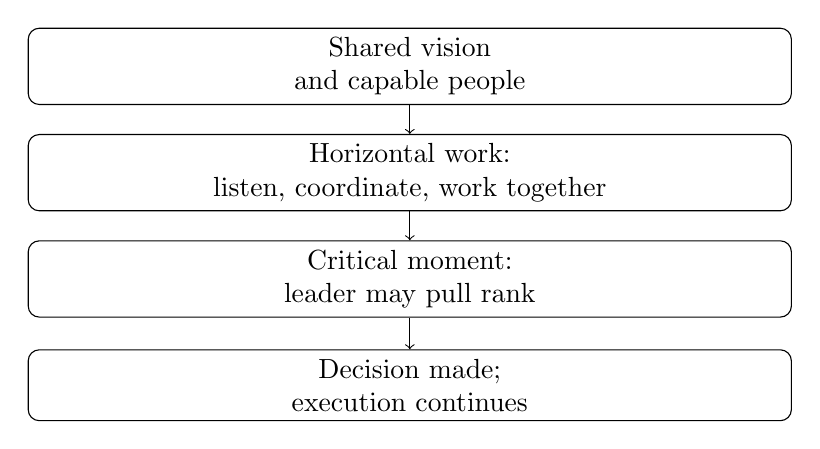
\begin{tikzpicture}
\node[draw, rounded corners, align=center, text width=0.78\linewidth] at (0,0) (vision) {Shared vision\\and capable people};
\node[draw, rounded corners, align=center, text width=0.78\linewidth] at (0,-1.35) (table) {Horizontal work:\\listen, coordinate, work together};
\node[draw, rounded corners, align=center, text width=0.78\linewidth] at (0,-2.70) (rank) {Critical moment:\\leader may pull rank};
\node[draw, rounded corners, align=center, text width=0.78\linewidth] at (0,-4.05) (execute) {Decision made;\\execution continues};
\draw[->] (vision) -- (table);
\draw[->] (table) -- (rank);
\draw[->] (rank) -- (execute);
\end{tikzpicture}
\caption{A transcript-backed reconstruction of the management rule: collaboration is the default, but decisive authority remains available in critical moments.}
\end{figure}

The scaling mechanism is social before it is numerical. Surround yourself with professionals or aspiring professionals, share the vision, and listen. The speaker's complaint is that people are too ready to fight, and that posture should not enter the business.

\section{The Method: Ask Everywhere, Then Learn Fast}

After a declined interview, the hosts pause to reveal the operating method behind the video. They ask everywhere: at the mall, at the ice cream shop, at the convenience store, in ordinary lines and ordinary streets. This is not a digression. It shows the practical side of opportunity creation. The interviews happen because someone keeps asking.

The next business thread comes from a VP of marketing at a software company. He says he started in many startups and had opportunities at larger companies, but the startup path let him touch many areas instead of being pigeonholed into one role. His claim is that breadth accelerated learning.

A compact way to preserve the point is:
\begin{equation}
\hbox{learning rate}
\quad \hbox{increases with} \quad
\hbox{role surface area}.
\end{equation}
This is not a measured law. It is a faithful summary of the interviewee's mechanism. More kinds of responsibility produced more opportunities to learn, and that learning compounded faster than an early comfortable job would have.

The money question returns, and he gives only a guarded answer: high six figures, really high six figures. The imprecision matters. Income is evidence, but the more durable evidence is his explanation of how the career acquired leverage.

\section{Relationships: Access Is Not The Same As Value}

The same VP answers another repeated question: what matters more, what you know or who you know? His answer is direct: who you know. He adds that relationships in the role you are already in can lead to additional roles later, and that one should remember that one is a brand. The claim is not merely that networking works. It is that every interaction may become part of a future opportunity set.

Then the next speaker sharpens the question. He says it matters to surround yourself with millionaires, billionaires, and people ten steps ahead. But once you are in those circles, you must provide value. Otherwise the relationship does not continue.

\subsection{Question \& Answer}

\paragraph{Question.}
Is success about who you know, or what you can do?

\paragraph{Answer.}
The transcript resolves the tension sequentially. Relationships may get the door open; value keeps the relationship alive. A compact model is:
\begin{equation}
\hbox{durable relationship}
\approx
\hbox{access}
+
\hbox{provided value}.
\end{equation}
Access without contribution is fragile. Skill without access may remain unseen. The useful business position combines the two: we enter the room through relationship, and we remain there by being useful.

This is why the interviewee's harsher line matters even after softening the language: if you bring nothing to the table, you should not expect the table to keep making room for you.

\section{Self-Employment, Risk, And The Market's Indifference}

The next medical-business owner refuses to disclose exact income, but answers that it was ``a lot.'' He says he has been in medical for \(26\) years and owns his own business. Then he gives the harder lesson: working for yourself is not for everybody.

His concrete claim is that he has owned a stem cell company for \(17\) years and has a business doing more than \(4\) million in revenue:
\begin{equation}
R > \$4{,}000{,}000.
\end{equation}
We must keep that as revenue. It is not profit, owner income, valuation, or cash available to spend. The correct reading is:
\begin{equation}
R = \hbox{top-line business activity},
\qquad
\Pi = R - \hbox{costs}.
\end{equation}
The transcript does not give the costs, so it does not give \(\Pi\).

His advice is competitive and unsentimental. Take chances. After the first year out of school, he says, nobody cares much where you went. Then it becomes you against the rest of the market. His father's advice adds the sales mechanism: people buy from people they like. That is anecdotal, but it points to a durable commercial fact. Trust lowers friction. Likability, reliability, and confidence can become economic assets when they help a buyer choose.

The other piece of inherited advice is attention discipline: control the controllables. In business terms, the scarce resource is not only money. It is also focus. If a variable cannot be acted on, worrying over it does not improve the system.

\section{Assets, Liquidity, And Strategic Timing}

The next major turn is from income to ownership of assets. A former military professional describes buying a house at one duty station, moving, buying another, and renting the previous one out. Without initially thinking of himself this way, he became an investor. By the time of the interview, he says:
\begin{equation}
N_{\mathrm{properties}} = 4.
\end{equation}

He also describes himself as cash poor and asset rich. That phrase is worth slowing down for. It distinguishes wealth on a balance sheet from cash available now:
\begin{equation}
\hbox{net worth}
=
\hbox{liquid cash}
+
\hbox{illiquid assets}
-
\hbox{liabilities}.
\end{equation}
Real estate can appreciate, produce rent, and serve as collateral, but it is not the same thing as cash in hand.

\paragraph{Worked example.}
Suppose a person owns real estate worth \(A\), owes liabilities \(L\), and has liquid cash \(C\). Then:
\begin{align}
W &= C + A - L,\\
\hbox{liquid position} &= C.
\end{align}
The person can have large wealth \(W\) and still have a tight liquid position if \(C\) is small. Selling an asset may increase \(C\), but it also changes \(A\), may trigger costs or taxes, and may remove future rent. Refinancing may increase \(C\), but it also changes \(L\). That is the mechanical content of being cash poor and asset rich.

The speaker says he is preparing to offload all the properties and reposition for a coming recession. He hopes to go into things that may return \(5x\) through \(10x\):
\begin{equation}
5x \leq \hbox{target multiple} \leq 10x.
\end{equation}
This must stay attributed and speculative. The lesson is not that those returns are guaranteed. The lesson is that asset owners face a timing problem: what to hold, what to liquidate, and when to exchange one exposure for another.

\section{Create, Fix, Replicate, And Work Backward}

When asked for the blueprint to becoming a millionaire, the same speaker refuses to pretend that sixty seconds can contain the whole answer. Then he gives a compact rule: create. Do not simply wake up and go with the flow. Live strategically. Create a YouTube channel, create a product, find something broken and fix it, or recreate something that already works in one's own format.

\begin{figure}
\centering
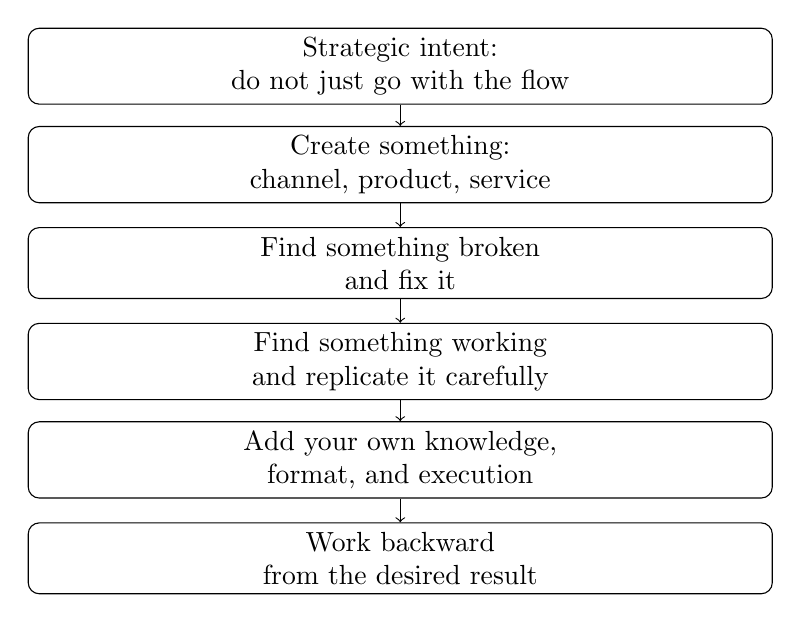
\begin{tikzpicture}
\node[draw, rounded corners, align=center, text width=0.76\linewidth] at (0,0) (intent) {Strategic intent:\\do not just go with the flow};
\node[draw, rounded corners, align=center, text width=0.76\linewidth] at (0,-1.25) (create) {Create something:\\channel, product, service};
\node[draw, rounded corners, align=center, text width=0.76\linewidth] at (0,-2.50) (fix) {Find something broken\\and fix it};
\node[draw, rounded corners, align=center, text width=0.76\linewidth] at (0,-3.75) (copy) {Find something working\\and replicate it carefully};
\node[draw, rounded corners, align=center, text width=0.76\linewidth] at (0,-5.00) (spin) {Add your own knowledge,\\format, and execution};
\node[draw, rounded corners, align=center, text width=0.76\linewidth] at (0,-6.25) (plan) {Work backward\\from the desired result};
\draw[->] (intent) -- (create);
\draw[->] (create) -- (fix);
\draw[->] (fix) -- (copy);
\draw[->] (copy) -- (spin);
\draw[->] (spin) -- (plan);
\end{tikzpicture}
\caption{A transcript-backed reconstruction of the creation rule: create, fix, or replicate, then add differentiated execution and plan backward.}
\end{figure}

The next entrepreneur makes the risk more personal. He describes sitting in a Texas A\&M construction science classroom, already seeing the job path ahead, and deciding he had to jump. His junk removal company became a demolition company and then a land-clearing company. He says he started at \(21\), is \(28\), and now has two other businesses.

His income claim is approximate:
\begin{equation}
I_{\mathrm{year}} \approx \$650{,}000.
\end{equation}
But he immediately adds the volatility:
\begin{equation}
I_{\mathrm{month}} \in \{\$75{,}000,\ \$10{,}000,\ldots\}.
\end{equation}
This is one of the chapter's most useful quantitative moments. A large annual number can hide uneven monthly cash flow. Entrepreneurship often exchanges salary smoothness for upside, uncertainty, and variance.

The same speaker then returns to assets and planning. He recommends getting control of real estate early if possible, even with help from parents, because an owned asset can appreciate, help build credit, produce rent, and remain present even if a business fails. Then he gives the construction version of working backward: if he wants to build pools, he asks which mechanical, electrical, plumbing, gunite, shotcrete, and concrete pieces are required; who does them; where they are; and how good they are. The plan begins at the end and decomposes the path.

\section{Credentials, Buckets, And Transferable Skill}

The final interviews move from entrepreneurial ownership into durable financial structures and transferable training. A retired law-enforcement professional says he spent about \(30\) years with the Los Angeles Police Department and at one point topped \(300{,}000\) dollars doing celebrity weddings and security:
\begin{equation}
I_{\mathrm{year}} \gtrsim \$300{,}000.
\end{equation}
His financial advice is to invest. The transcript is garbled around ``invest in diversity'' and ``pension in a divert,'' but the meaning is clear enough to state cautiously: he describes not depending only on a pension, but also using a deferred compensation program. He calls them two buckets one can draw on when older:
\begin{equation}
\hbox{retirement resources}
=
\hbox{pension}
+
\hbox{deferred compensation}.
\end{equation}
This is not a contribution formula. It is a structural rule: one bucket is more fragile than two, especially when the second is built by disciplined deferral.

The last speaker has an electrical engineering degree but works in cybersecurity and privacy. Asked for his best financial decision, he does not name a trade, a stock, or a house. He names engineering. Even when one does not work as an engineer, he says, the training opens other areas because it teaches problem solving.

That is the last turn of the lecture. The question began as income. It ends as capability. What do we own? What can we solve? What relationships can we sustain by providing value? What structures do we build so that one job, one client, or one month does not determine the whole future?

\section{Summary}

The evidence in this chapter is interview evidence rather than blackboard mathematics. Still, the quantitative spine is clear. We separate personal income from revenue and profit. We separate net worth from liquid cash. We treat debt as capital plus obligation. We treat networking as access plus value. We treat annual income as the output of a business system, not as a simple salary number.

The recurring lesson is ownership under uncertainty. Some speakers own businesses, some own properties, some own relationships, some own skills, and some own disciplined financial buckets. The income question opens the conversation, but the durable chapter is about the mechanisms that make income possible and the structures that keep it from disappearing.